\paragraph{}This chapter will explain the methodology and requirements for the \ac{SLAM} tuning module, developed for \ac{RUSTLE}. For each implemented tuning technique, a high level overview of its architecture is provided. Test settings, including test algorithms and dataset choices, are also justified.

\begin{figure}[h]
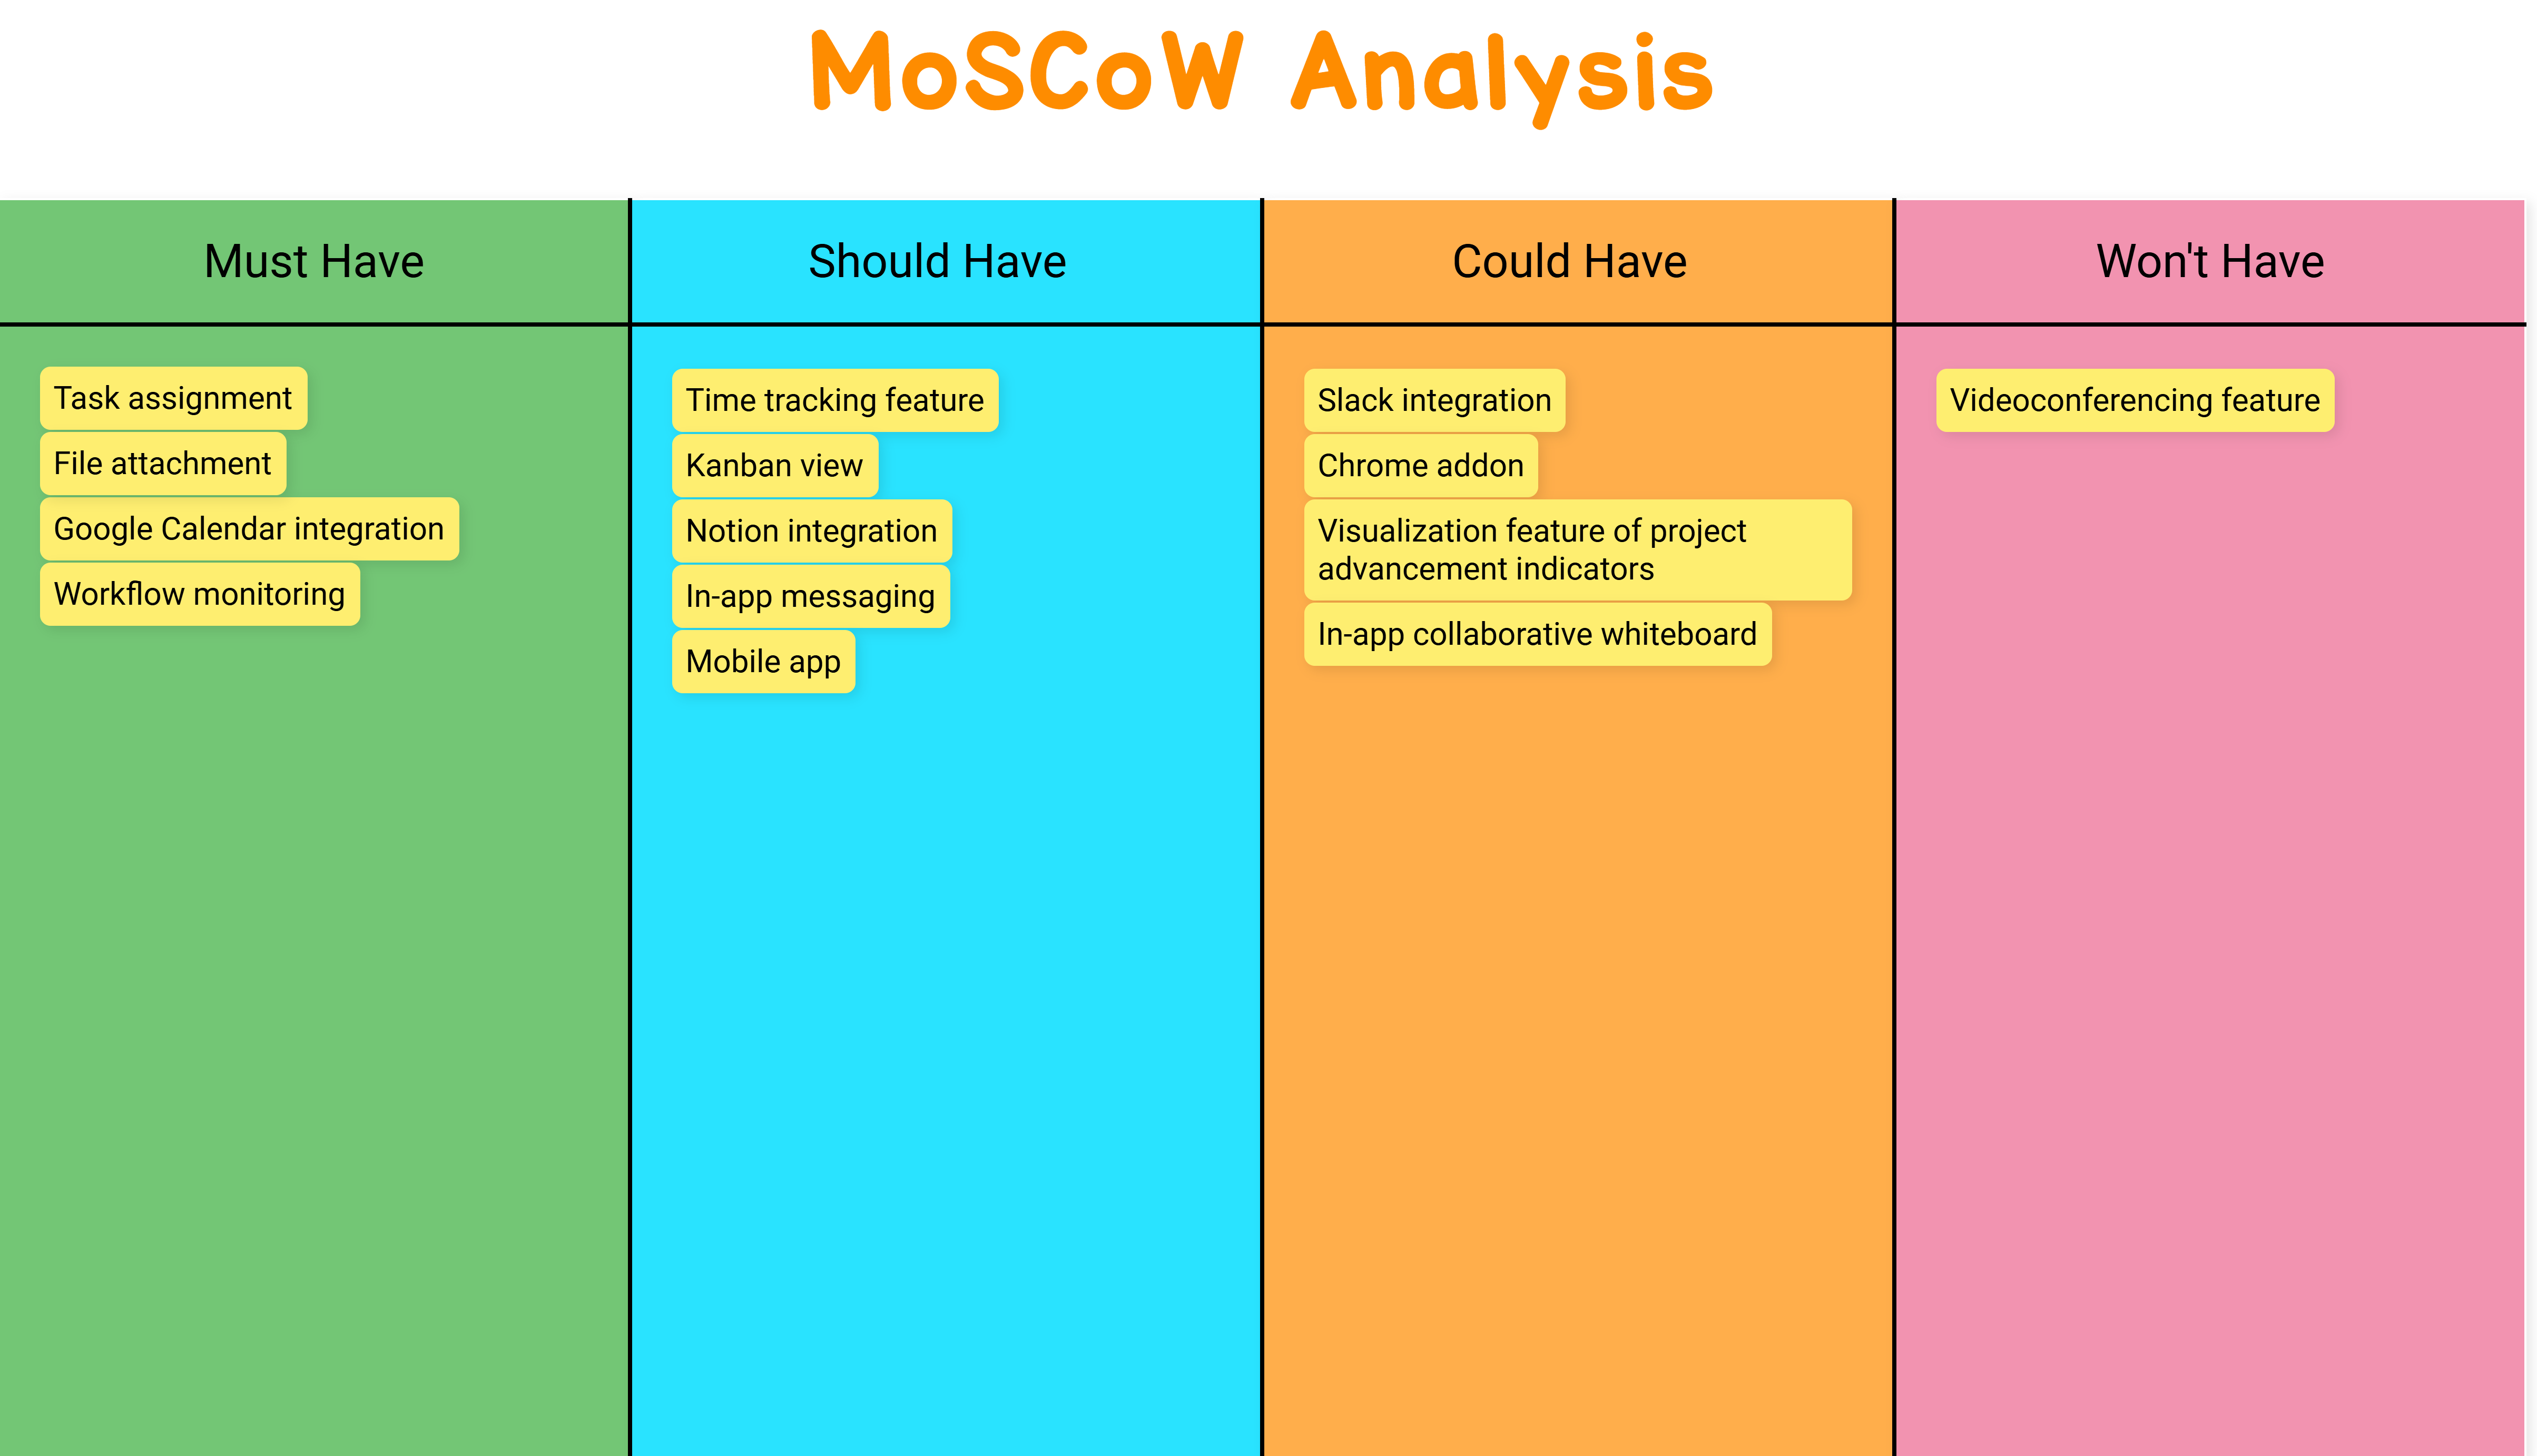
\includegraphics[width=0.85\linewidth]{images/moscow.png}
\end{figure}

\section{\ac{RUSTLE}}

\paragraph{}\ac{RUSTLE} is a command line application, written in Rust, which facilitates the process of running localization experiments. On a high level, it allows to run different SLAM algorithms on different datasets, with user defined hyperparameters.

\section{Grid Search}

\section{Random Search}

\section{Simulated Annealing}

\section{Testing}

\subsection{Algorithms}

\subsection{Datasets}